\documentclass[a4paper, 11pt]{scrreprt}
\usepackage[utf8]{inputenc}
\usepackage[ngerman]{babel}
\usepackage[T1]{fontenc}
\usepackage{lmodern}
\usepackage{amsmath,amssymb,amstext,amsfonts,mathrsfs}
\usepackage{graphicx}
\usepackage{color}

\usepackage{marginnote}

\pagestyle{headings}

\newtheorem{defi}{Definition}[section]
\newtheorem{prop}[defi]{Proposition}
\newtheorem{satz}[defi]{Satz}
\newtheorem{koro}[defi]{Korollar}
\newtheorem{lemma}[defi]{Lemma}

\newenvironment{beweis}[1][Beweis]{\begin{trivlist}
	\item[\hskip \labelsep {\bfseries #1}]}
	{\end{trivlist}}

\newcommand{\RR}{\mathbb{R}}
\newcommand{\EE}{\mathbb{E}}
\newcommand{\ZZ}{\mathbb{Z}}
\newcommand{\NN}{\mathbb{N}}
\newcommand{\FF}{\mathcal{F}}

\newcommand{\student}[1]{\marginnote{{\normalfont\bf #1}}}

\title{Fallstudien der math. Modellbildung}
\author{Manuela Lambacher, Dominik Otto, Andreas Wiedemann}
\date{\today}

\begin{document}
\parindent 0pt
\maketitle
\tableofcontents

\chapter{Whittaker-Shannon Interpolation Theorem}

\section{The Whittaker-Shannon Interpolation Theorem}
If \(x \in L^2(\RR^d)\) is a \(\omega\)-bandlimited function, there exists a \(\tau_0 > 0\) such that for all \(\tau \in \left(0,\tau_0\right]\)
\[x(t) = \sum_{k \in \ZZ^d} x(\tau k) \prod_{i=1}^d sinc\left(\frac{t_i-k_i \tau_i}{\tau_i}\right).\]

\section{Proof of the Theorem}
Define \(\tau_0 = \frac{1}{\omega} := \left(\frac{1}{\omega_0}, \ldots, \frac{1}{\omega_d}\right)\) and choose \(\tau \in (0,\tau_0]\) arbitrarily. \\
Besides denote \(\Omega := \prod_{i=1}^d \left[-\frac{1}{2}\omega_i ,\frac{1}{2}\omega_i\right]\) and \(T := \prod_{i=1}^d \left[-\frac{1}{2\tau_i} ,\frac{1}{2\tau_i}\right]\).
% \(X(f) := \FF(x)(f) = \int_{\RR^d} x(t) e^{-2\pi itf} dt\)

\begin{equation}
x \in L^2_w(\RR^d) \Rightarrow \forall f\notin \Omega: \FF(x)(f) = 0
\end{equation}

The consequence of this condition and of the linearity of \(\FF(x)\) is:

\[\forall f\in T, k \in \ZZ^d: \FF(x)\left(f+\frac{k}{\tau}\right) = \FF(x)(f) + \FF(x)\underbrace{\left(\frac{k}{\tau}\right)}_{\notin \Omega} = \FF(x)(f)\]

Thus the formula can be rewritten.

\begin{equation}
\forall f \in \Omega_{\omega}: \FF(x)(f) = \sum_{k \in \ZZ^d} \FF(x)\left( f+\frac{k}{\tau}\right)
\end{equation} 

(1.1) and (1.2) allow us to say:

\[\FF(x)(f) = \chi_{T}(f) \sum_{k \in \ZZ^d} \FF(x)\left(f+\frac{k}{\tau}\right)\]

With the aid of the Poisson summation formula (Theorem 0.3) you can conclude:
\begin{equation}
\FF(x)(f) = \chi_{T}(\tau f) \det(\tau) \sum_{n \in \ZZ^d} x(n\tau)e^{-2\pi i n\tau f}
\end{equation}

Mit dieser Poissonschen Summenformel habe ich ziemliche Probleme:\\
Macht unsere Notation im Skript da Sinn, bzw. wie soll das mit \(k,n \in \ZZ^d\) fuktionieren? Außerdem haben wir auch ganz andere Vorraussetzungen, als z.B. bei Wikipedia, da muss die Funktion u.a. in \(C^{\infty}\) liegen! \\
Wir müssen auch klären, ob wir die Poisson-Regel überhaupt anwenden dürfen, die Stetigkeit, bzw. die beliebige diff'barkeit ergeben sich mir jetzt nicht so, laut dieser Bemerkung am Ende von Übung 3 geht es ja aber...\\
Und schließlich an Andi: Hast du die Formel richtig angewandt? Wo kommt das \(\det{\tau}\) her? Ich würde auch sagen, dass im Exponent kein Minus steht? \\
Das ist echt ein kack, aber bis auf diesen Schritt finde ichs ziemlich gut :) Bist du da selbst drauf gekommen oder hast du das iwo aus dem Internet? Falls letzteres, könntest du uns den Link schicken?\\


Now we want to prove that \(\FF\left( \prod_{j=1}^d sinc \left( \frac{t_j-n\tau_j}{\tau_j}\right)\right)(f) = \det(\tau)\chi_{T}(\tau f)e^{-2\pi in\tau f}\).

\begin{align*}
\FF^{-1}\left( \det(\tau) \chi_{T}(\tau f) e^{-2 \pi i n \tau f}\right) 
&= \int_{\RR^d} \det(\tau) \chi_{T}(\tau f) e^{-2 \pi i n \tau f} e^{2 \pi i f t} df \\
&= \int_{\RR^d} \det(\tau) \chi_{T}(\tau f) e^{2 \pi i f (t-n\tau) }df \\
&= \int_{-\frac{1}{2\tau_1}}^{\frac{1}{2\tau_1}} \cdots \int_{-\frac{1}{2\tau_d}}^{\frac{1}{2\tau_d}} \prod_{j=1}^d \tau_j e^{2 \pi i f_j(t_j-n \tau_j)}df_1 \ldots df_d \\
&= \prod_{j=1}^d \int_{-\frac{1}{2\tau_j}}^{\frac{1}{2\tau_j}} \tau_j e^{2 \pi i f_j (t_j - n \tau_j)}df_j \\
&= \prod_{j=1}^d \left[  \frac{\tau_j}{2 \pi i (t_j - n \tau_j)} e^{2 \pi i f_j (t_j - n \tau_j)} \right]_{f_j = -\frac{1}{2\tau_1}}^{\frac{1}{2\tau_1}} \\
&= \prod_{j=1}^d \frac{\tau_j}{2 \pi i (t_j - n \tau_j)} \left( e^{\pi i \frac{t_j - n \tau_j}{\tau_j}} - e^{-\pi i \frac{t_j - n \tau_j}{\tau_j}} \right) \\
&= \prod_{j=1}^d sinc \left( \frac{t_j - n \tau_j}{\tau_j} \right)
\end{align*}
tabelle
Hence formula (1.3) is:

\[\FF(x)(f) = \sum_{n \in \ZZ^d} x(n\tau) \FF\left(\prod_{j=1}^d sinc \left( \frac{t_j - n \tau_j}{\tau_j} \right) \right)(f)\]

Through applying the inverse transform on both sides, the theorem is proved.

\begin{align*}
x(t) = \FF^{-1}(\FF(x))(t) &= \FF^{-1} \left( \sum_{n \in \ZZ^d} x(n \tau) \FF \left( \prod_{j=1}^d sinc \left( \frac{t_j - n \tau_j}{\tau_j} \right) \right) \right) \\
&= \sum_{n \in \ZZ^d} x(n\tau) \prod_{j=1}^d sinc \left( \frac{t_j - n \tau_j}{\tau_j} \right)
\end{align*}

\section{Meaning, real-life applications and limitations}

\chapter{Das Marchenko-Pastur-Gesetz}

\section{Das Marchenko-Pastur-Gesetz}

Sei \(Y_N\) eine \(N\times M(N)\)-Matrix mit unabhängigen zentrierten Einträgen mit Varianz \(1\),
	\[\sup_{j,k,N} \EE\left[ | Y_N(j,k)|^q\right] = C_q < \infty \qquad \forall q \in \NN\]
und \(M(N) \in \NN\) so, dass
	\[\lim_{N\to\infty} \frac{M(N)}{N} = \alpha \in[1,\infty). \]
Sei weiterhin die Wishart-Matrix gegeben als 
	\[W_N = \frac{1}{N}Y_NY_N^T,\]
und habe die empirische Eigenwertverteilung
	\[L_N = \frac{1}{N} \sum_{j=1}^{N} \delta_{\lambda_j} \]
und das Zustandsdichtemaß \(\overline{L_N} = \EE[L_N]\). Dann gilt die Konvergenz
	\[\overline{L_N} \xrightarrow{\text{w}} f_{\alpha}(x)dx \quad(N\to\infty)\]
im Raum der Wahrscheinlichkeitsmaße auf \(\RR\), wobei
	\[f_{\alpha}(x)=\frac{1}{2\pi x}\sqrt{(x-(1-\sqrt{\alpha})^2_{+}((1+\sqrt{\alpha})^2_{+}} \]

\newpage
\section{Beweis des Marcenko-Pastur Gesetzes}
Zuerst bringen wir \(N^{l+1} \langle \overline{L_N}, x^l \rangle\) in eine Form, die eine weitergehende Untersuchung ermöglicht:
\begin{equation}
\begin{split}
		N^{l+1} &\langle \overline{L_N}, x^l \rangle\ 
		= N^{l+1} \cdot \int x^l \overline{L_N}(dx) 
		= N^{l+1} \cdot \frac{1}{N} \cdot \EE[tr(W^l_N)] 
		= N^l \sum_{j_1,...,j_l = 1}^N \EE\left[\prod_{p = 1}^l W_{j_p,j_{p+1}}\right] \\
		&= N^l \sum_{j_1,...,j_l = 1}^N \EE\left[\prod_{p = 1}^l \frac{1}{N} \sum_{k = 1}^{M(N)} Y_N(j_p,k) \cdot Y_N(j_{p+1},k) \right] \\
		&= \sum_{j_1,...,j_l = 1}^N \EE \left[\left(\sum_{k = 1}^{M(N)} Y_N(j_1,k) \cdot Y_N(j_2,k)\right) \cdot \left(\prod_{p = 2}^l \sum_{k = 1}^{M(N)} Y_N(j_p,k) \cdot Y_N(j_{p+1},k) \right) \right] \\
		&= \sum_{j_1,...,j_l = 1}^N \EE\left[	\prod_{p = 2}^l \sum_{k_1,k_2 = 1}^{M(N)} Y_N(j_1,k_1) \cdot Y_N(j_2,k_1) \cdot Y_N(j_p,k_2) \cdot Y_N(j_{p+1},k_2) \right] \\
		&= ... \\
		&= \sum_{j_1,...,j_l = 1}^N \sum_{k_1,...,k_l = 1}^{M(N)} \EE[Y_N(j_1,k_1) Y_N(j_2,k_1) Y_N(j_2,k_2) Y_N(j_3,k_2) ... Y_N(j_l,k_l) Y_N(j_1,k_l)]\\
 &= \sum_{r_1,r_2 = 1}^l \sum_{\substack{J:v(J)=r_1\\ K:v(K)=r_2 }} \EE[Y_N(J,K)]
\end{split}
\end{equation}
wobei 
\begin{align*}
	&J=(j_1,j_2,j_2,...,j_l,j_l,j_1), K=(k_1,k_1,...,k_l,k_l),\\
	&v: \NN^{2l}\to \NN,\ v(X) := \text{Anzahl der verschiedenen Indizes in X}
\end{align*}
Die einzelnen Summanden können also als Eulergraphen auf \(r_1+r_2 \)Knoten und \(2l\) Kanten interpretiert werden.
Damit ergeben sich die drei Fälle (setze \(r = r_1+r_2\) )
\begin{itemize}
	\item \(r < l+ 1\)\\
		\begin{equation}
			\begin{split}
			\EE[Y_N(J,k)] &\leq \prod_{n=1}^l \left(\sup_{j,k,N}\EE\left[|Y_N(j,k)|^l\right]\right)^{\frac 1 l} \\
			& = \prod_{n=1}^l C_l^{\frac 1 l} = C_l
			\end{split}
			\end{equation}
	Außerdem gilt: 
		\begin{align}
			\#\{J: v(J)=r_1\} &\leq \begin{pmatrix} N \\ r_1 \end{pmatrix} r_1^l \leq N^{r_1}r_1^l \\
			\#\{K: v(K)=r_2\} &\leq \begin{pmatrix} M(N) \\ r_2 \end{pmatrix} r_2^l \leq M(N)^{r_2}r_2^l
		\end{align}
	Somit ergibt sich aus \((2.2) - (2.4)\): 
	\begin{equation}
		\frac {1}{N^{l+1}} \sum_{\substack{J:v(J)=r_1\\ K:v(K)=r_2 }} \EE[Y_N(J,K)] < C_l (l+1)^l \frac{N^{r_1} M(N)^{r_2}}{N^{l+1}} \xrightarrow{N\to\infty} 0
	\end{equation}
		
	\item \(r> l+1\) \\
		Nach Lemma aus der Vorlesung exisitert eine einfache, echte Kante und somit \(\EE[Y_N(J,K)]=0\), da die Matrixeinträge unabhängig sind.
	\item \(r=l+1\)\\
		Es tragen also nur die Graphen auf \(l+1\) verschiedenen Knoten zu \(\lim_{N\to\infty} \langle \overline{L_N}, x^l \rangle \) bei. Diese Graphen haben die Struktur eines Doppelbaumes%, denen man geordnete, nicht überkreuzende Paarzerlegungen und damit auch Catalanpfade zuordnen kann.
\end{itemize}
%\textbf{Weitere Analyse von \(\beta_l\):}\\
Diese Doppelbaumstruktur lässt sich wie folgt nutzen:\\
Wähle für einen Doppelbaum \(r\) Knoten aus den \(k\)-Knoten und \(l+1-r\) Knoten aus den \(j\)-Knoten. Dann folgt:
\begin{equation}
	\begin{split}
	\sum_{J,K: v(J)+v(K) = l+1} \EE[Y_N(J,K)] = &\sum_{r=1}^{l}\begin{pmatrix} N\\ l+1-r\end{pmatrix} (l+1-r)! \begin{pmatrix} M(N)\\r\end{pmatrix} r! \\
	&\cdot \#\{\text{Doppelbäume mit }l+1-r\ j\text{-Knoten und } r\ k\text{-Knoten}\} \\
	%=& \sum_{r=1}^{l} \begin{pmatrix} N\\ l+1-r\end{pmatrix} (l+1-r)! \begin{pmatrix} M(N)\\r\end{pmatrix} r! \cdot \begin{pmatrix} 2l-2\\2r-2\end{pmatrix} C_{l-r}
	\end{split}
\end{equation}
%Eine Formel für die Anzahl der Doppelbäume folgt aus der nachfolgenden Konstruktion (Anm: das -2 folgt immer, da die beiden Wurzelkanten fest 0 im Catalanpfad sind; Die Catalanzahl für l-r, weil von dem gesamten Pfad der Länge 2l 2r Stücke flach sind und die übrigen wie beim normalen Catalanpfad aufgeteilt werden können) \\ \\
Ein Doppelbaum mit \(r\  k\)-Knoten und \((l+1-r)\ j\)-Knoten kann wie folgt als Catalan-Pfad der Länge \(l\) interpretiert werden:\\
Wähle als Wurzel des Baumes einen \(j\)-Knoten und gliedere den Baum in Ebenen, wobei die Wurzel in der 0.Ebene liegt.(Die k-Knoten liegen also in ungeraden Ebenen, die j-Knoten in geradenen Ebenen) Verweise jede Kante mit einer Richtung, sodass bei jeder Doppelkante eine Kante von dem Knoten wegführt und eine zu ihm hinführt. Konstruiere den Catalan-Pfad wie folgt:\\
\begin{itemize}
	\item Alle Kanten zwischen der Wurzel und der ersten Ebene sind Flachstücke: \((+0)\)
	\item Wenn eine Kante von ungerader Ebene aufwärts auf gerade Ebene führt: \((+1)\)
	\item Wenn eine Kante von gerader Ebene abwärts auf ungerade Ebene führt: \((-1)\)
	\item Die restlichen Kanten sind alle Flachstücke: \((+0)\)
\end{itemize}
Beispiel: \\
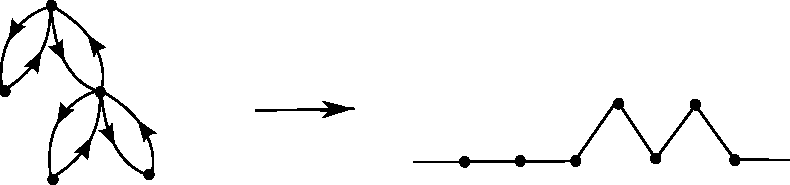
\includegraphics{Catalan-Pfad}
Lässt man die Wurzel außen vor, liegen \(r\ k\)-Knoten in den ungeraden Ebenen und \(l-r\ j\)-Knoten in den geraden Ebenen. Damit ergibt sich aus dieser Konstruktion, dass \(l-r\) die Anzahl der Aufstiege (und Abstiege) und \(2r\) die Anzahl der Flachstücke im Catalan-Pfad sind.  Denn: zu jedem \(j\)-Knoten führt genau eine Kante aus einer unteren Ebene hin und es führt genau eine Kante in eine untere Ebene zurück (Doppelbaum!). \\
\\ Die Abbildung von den Doppelbäumen auf die Catalanpfade ist eine Bijektion, da:
\begin{itemize}
 \item[•]Da der Graph eulersch ist, ist $ \sum_{i=1}^{2l} $ =0; Der Graph ist immer über 0, ansonsten würde es ein m geben, sodass $ \sum_{i=1}^{2m-1}s^{i}=-1, ~\sum_{i=1}^{2m}s^{i}=0, ~ s_{2m-1}=-1  $. Also könnten wir einen Doppelbaum mit Knoten {1,2,...2m} konstruieren, und da $ s_{2m-1}=-1  $ ist, würde eine Kante von diesem Knoten zurück zu einem der ersten 2m Knoten gehen, was dem Aufbau eines Doppelbaums widersprechen würde. Insgesamt haben wir also einen Catalanpfad konstruiert. 
 \item[•] Surjektivität:  für jeden Catalanpfad der Länge l der Form $\lbrace s_{i} \rbrace$, $ i \leq 2l, i \in \NN $ kann ein Doppelbaum als Urbild wie folgt konstruiert werden: für i gerade: $s_{i}=-1 \rightarrow $ gehe von $j_{i/2}$abwärts, bei $s_{i}=0  $ aufwärts; für i ungerade bei $s_{i}=1 $ aufwärts, bei $s_{i}=0 $ abwärts. 
\item[•] Injektivität analog zur Übung (bzw muss man das unbedingt nochmal zeigen?)\\
\end{itemize}
Die betrachteten Doppelbäume haben s.o. ein kombinatorisches Gewicht von 
	\begin{equation}
		\begin{pmatrix} N\\ l+1-r\end{pmatrix} (l+1-r)! \begin{pmatrix} M(N)\\r\end{pmatrix} r!
	\end{equation}
Für N hinreichend groß ist dies genähert \(N^{l+1-r}M(N)^r\). Damit folgt:
	\begin{equation}
		\frac {1}{N^{l+1}} N^{l+1-r}M(N)^r =~ \left( \dfrac{M(N)}{N}\right)^{r}\to \alpha^r
	\end{equation}
und damit:
	\begin{equation}
	\begin{split}
		\beta_l &:= \lim_{N\to\infty} \langle \overline{L_N}, x^l \rangle\\
		&= \lim_{N \to \infty} \sum_{J,K: v(J)+v(K) = l+1} \dfrac{1}{N^{l+1}}\EE[Y_N(J,K)] = \sum_{r=1}^{l} \alpha^r\ \begin{pmatrix} 2l-2\\2r-2\end{pmatrix} C_{l-r} \\
		&= \sum_{r=1}^{l} \sum_{p_{r} \in C_{l}} \alpha^{r} = \sum_{p\in C_l} \alpha^r
	\end{split}
	\end{equation}

wobei \(r = \frac 1 2 \#\{\text{Flachstücke in }C_l\} = l  - \#\{\text{Anstiege in }  C_l\}\), und $ p_{r} $ Catalanpfad mit 2r Flächenstücken.\\



An Manu: kannst du diese Formel für \(\beta_l\) genauer erklären? Ich verstehe nicht wirklich, was du da machst...\\


Mach ich. Also ich hab lang nicht verstanden, was das Kombinatorik-zeug vorne dran mit den Catalanpfaden zu tun hat. Du hattest glaub ich $C_l$ als Anzahl der Catalanpfade. Beim Überlegen für (10) dem nächsten Punkt hab ich mir dann die Formel für die Pfade gebaut, die im Grunde nur auf deiner Konstruktion basiert (und von der bist du ja hoffentlich überzeugt:) )\\
$ \longrightarrow $Also wir brauchen die Anzahl der Catalanpfade, durch die wir unsere Doppelbäume beschreiben, weil's eine Bijektion ist. Nur haben wir andere Catalanpfade als die normalen:)\\
Die Catalanpfade, die wir in der Vorlesung gebaut haben, mit der Anzahl $C_l$ (Catalanzahlen), sind dadurch definiert, dass du bei jedem Schritt + oder - 1 gehst, und das nichtüberkreuzend. \\ Bei unseren Catalanpfaden hast du aber noch deine "Flachstücke" mit 0 eingebaut! Und zwar 2r von denen. Also wie viele gibts von denen für ein bestimmtes r? Nach Konstruktion mit einem Knoten, sagen wir mal den j1, als Wurzel, sind der erste und letzte Schritt in dem Pfad auf jeden Fall flach, also 0. Da gibt's keine andere Möglichkeit. Von den restlichen 2l-2 Schritten im Pfad sind noch 2r-2 flach, die suchen wir als erstes raus. Das macht dann die $\begin{pmatrix} 2l-2\\2r-2\end{pmatrix} $.\\ 
Bleiben uns noch 2l-2-(2r-2) Schritte übrig, die mit +/-1 zu belegen sind. Und zwar nichtüberkreuzend. Was das gleiche ist wie wenn du einen l-r-langen Catalanpfad bauen willst, weil du die 2r Flachstücke einfach mal ignorierst, die ändern ja nichts. Daher kommt das $ C_{l-r} $. Und wir haben die Anzahl!\\ Über r aufsummieren, damit wir alle Fälle mit r Knoten aus M(N), Rest aus N, haben. Das übrige Kombinatorik-zeug ist ja $\alpha^r  $, und schon steht die Formel da\\
Die Formel für die Anzahl der Catlanpfade ist ganz praktisch für (10), für $ \beta$ selber brauchen wir sie ja erst mal nicht, deshalb wieder umcshreiben in $ \sum_{r} \alpha^{r} \#\{ \text{Catalanpfade mit 2r Flachstücke} \}$. Wenn du sie mal die Anzahl nimmst, kannst auch über alle 2r-Catalanpfade aufsummieren, das hoch r ändert sich ja nicht. Und dann $= \sum_{r=1}^{l} \sum_{p_{r} \in C_{l}} \alpha^{r} = \sum_{p\in C_l} \alpha^r $.\\ \\
kurze Erklärung der Schritte schreib ich auch noch irgendwann oben rein.\\
 -> Danke für die Erklärung, davon sollten wir einiges in die spätere Endfassung ausfnehmen, damit die Formeln klarer werden! Was ich vllt hätte hinschreiben sollen ist, dass es bei mir beim vorletzten = hakt, also da, wo du die \(p_r\) einführst... \\ Jetzt mit richtiger Defintion von $ p_r $ klarer? \\

%\textbf{Beweis von  $\beta_{l}= \alpha \gamma_{l}$:}
Mit \(\beta_0 :=1, \gamma_0:=1 \) und
\begin{equation*}
		\gamma_l:=\sum_{p\in C_l} \alpha^{l-r} \qquad (l\geq 1)
\end{equation*}
gelten die Relationen
\begin{equation}
	\beta_l = \alpha\gamma_l=\alpha\sum_{r=0}^{l-1}\beta_r \gamma_{l-1-r}
\end{equation}
für alle \(l\geq 1\):
\begin{itemize}
	\item \begin{equation}
	\begin{split}
\alpha \gamma_{l} =& \sum_{p \in C_l} \alpha^{l+1-r},\\
\beta_l - \alpha \gamma_l =& \sum_{r=1}^{l} \alpha^r\ \begin{pmatrix} 2l-2\\2r-2\end{pmatrix} C_{l-r} - \sum_{r=1}^{l} \alpha^{l+1-r}\ \begin{pmatrix} 2l-2\\2l-2r\end{pmatrix} C_{r-1}   \\ 
\underset{\text{Symmetrie Binom.}}{=}& \sum_{r=1}^{l} \begin{pmatrix} 2l-2\\2l-2r\end{pmatrix} \left( C_{l-r} \alpha^r - C_{r-1}\alpha^{l+1-r} \right) \\
\overset{!}{=}& 0 \\
\end{split}
\end{equation}
Für die einzelnen Summenglieder folgt:
\begin{align*}
\text{i-tes Summenglied:} &\begin{pmatrix} 2l-2\\2l-2i\end{pmatrix} \left( C_{l-i} \alpha^i - C_{i-1}\alpha^{l+1-i} \right) \\
\text{(l+1-i)-tes Summenglied:}& \begin{pmatrix} 2l-2\\2l-2-2l+2i\end{pmatrix} \left( C_{l-1-l+i} \alpha^{l+1-i} - C_{1+l-i-1}\alpha^{l+1-1-l+i} \right)\\
 &= - \text{i-tes Summenglied}  
\end{align*}
Ist l gerade, dann heben sich folglich alle Summenglieder weg und die Summe ist 0, ist l ungerade, bleibt nur das (l+1)/2-te Summenglied übrig:
\begin{align*}
 &\begin{pmatrix} 2l-2\\l+1-2\end{pmatrix} \left( C_{l-\frac{l+1}{2}} \alpha^{\frac{l+1}{2}} - C_{\frac{l+1}{2} -1}\alpha^{l+1-\frac{l+1}{2}} \right)\\
&=\begin{pmatrix} 2l-2\\l-1\end{pmatrix} \left( C_{\frac{l-1}{2}} \alpha^{\frac{l+1}{2}} - C_{\frac{l-1}{2}}\alpha^{\frac{l+1}{2}} \right)=0
\end{align*}

Damit gilt der erste Teil von \((2.10)\)\\
\item
Die Konstruktion der Catalan-Pfade aus der Doppelbaumstruktur ermöglicht eine weitere Interpretation von \(r\) bzw. \(l-r\):\\
\begin{align*}
	r&=\# \{\text{Schritte von gerader Ebene zu \underline{höherer} ungerader Ebene}\} \\
	l-r &= \#\{\text{Schritte von ungerader Ebene zu \underline{höherer} gerader Ebene}\}
\end{align*}
Für die Catalan-Pfade ergibt sich dann, dass die zu \(r\) gehörigen Elemente immer an ungeraden Positionen und die zu \(l-r\) gehörigen Elemente immer an geraden Positionen liegen. (Wichtig für später).\\
Die Konstruktion der Pfade bedingt, dass das erste und letzte Element immer Flachstücke sind, sie können für die folgenden Überlegungen also vernachlässigt werden (wir betrachten also Catalan-Pfade der Länge \(l-1\) und erhalten eine Formel für \(\beta_{l-1}\) ). Sei \(2j\) die Stelle, an der zum ersten Mal die \(0\) erreicht wird. Falls \(j\not=0\) lässt sich der Pfad in zwei Teilpfade \(P_1, P_2\) der Länge \(2j\) und \(2l-2-2j\) aufteilen.\\
\(P_2\) ist dabei ein beliebiger Catalan-Pfad, also von der Form \(C_{l-1-j}\). \(P_1\) hat die Besonderheit, dass er erst an der letzten Position zur \(0\) zurückkehrt. Damit folgt, dass das erste und letzte Element festgelegt sind als aufsteigende bzw. absteigende Kante. Löscht man diese ebenfalls und subtrahiert von allen übrigen Elementen \(1\), so bleibt ein beliebiger Catalan-Pfad \(\tilde{P}_1\) der Länge \(2j-2\), also von der Form \(C_{j-1}\) übrig. \\
Die Kanten, die im Pfad \(\tilde{P}_1\) an gerader/ungerader Position sind, sind auch im ursprünglichen Pfad an gerader/ungerader Position, da die ersten beiden Kanten gelöscht wurden. Für \(P_2\) hat sich diese Eigenschaft aber genau vertauscht, man betrachtet nicht mehr die \(r\), sondern die \(l-r\) Kanten!\\
Daraus ergibt sich die Formel:
	\[\beta_{l-1}=\alpha \sum_{j=1}^{l-1}\beta_{j-1}\gamma_{l-1-j}\]
und damit
\begin{equation}
	\beta_l=\alpha \sum_{j=0}^{l-1}\beta_j\gamma_{l-1-j}
\end{equation}
Also gilt auch die zweite Relation von \((2.10)\).\\
\end{itemize}
(Ich muss zugeben, dass aus meiner Überlegung nicht klar wird, woher das zusätzliche \(\alpha\) kommt, daran arbeite ich noch ;) )

\textbf{Beweis von Formel (12)}\\
\begin{align*}
	Q_n :=& \alpha^{-1-n/2}\int_{\RR} f_{\alpha}(x)x(x-\alpha -1)^n\,\mathrm{d}x \\
	 =& \frac{1}{2\pi}\alpha^{-1-n/2} \int_{(1-\sqrt{\alpha})^2}^{(1+\sqrt{\alpha})^2} \sqrt{(x-(1-\sqrt{\alpha})^2)((1+\sqrt{\alpha})^2-x)} (x-\alpha -1)^n \,\mathrm{d}x\\
	=& \frac{1}{2\pi}\alpha^{-1-n/2} \int_{(1-\sqrt{\alpha})^2}^{(1+\sqrt{\alpha})^2} \sqrt{-\alpha^2+2\alpha x+2\alpha -x^2+2x-1}(x-\alpha-1)^n \,\mathrm{d}x\\
	\overset{x=y+\alpha+1}{=}& \frac{1}{2\pi}\alpha^{-1-n/2} \int_{-2\sqrt{\alpha}}^{2\sqrt{\alpha}} \sqrt{4\alpha -y^2} y^n \,\mathrm{d}y\\
	\overset{y=2\sqrt{\alpha}z}{=}& \frac{1}{2\pi}\alpha^{-1-n/2} \cdot 2^n \alpha^{n/2}\cdot4\sqrt{\alpha}\int_{-1}^{1} \sqrt{1-z^2}z^n \,\mathrm{d}z = \frac{2}{\pi} \cdot 2^n\int_{-1}^{1} \sqrt{1-z^2}z^n\,\mathrm{d}z \\
	\overset{\text{Übung 1}}{=}& \sigma(z^n) = \begin{cases} 0, &n\text{ ungerade}\\
	C_{\frac n 2}, &n\text{gerade} \end{cases}
\end{align*}
(Falls wir noch Platz füllen müssen, können wir hier die Rechnung aus der Übung auch wiederholen ;) )
Bei den "`Verständnis-Fragen"' habe ich jedoch etwas Probleme: \(f_{\alpha}\) ist für x=0 gar nicht definiert? Durch die Rechnung ergibt sich aber der Bezug zu \(\sigma(x)\), wo man dann doch beim Halbkreisgesetz wäre.\\
Zur Eindeutigkeit von \(f_{\alpha}\) sind diese "`verallgemeinerten Momente"' ein Problem. Habt ihr in der großen W-Theorie Vorlesung dazu was gemacht?\\

Finde nichts zu verallgemeinerten Momenten. Müssen wir am Dienstag fragen.\\
Ann: Theorem der Vorlesung auch für verallgemeinerte Momente anwendbar: f eind. bestimmt wenn $ Q_n< \infty $ (folgt aus (12)) und $ \sum_{n=0}^{\infty} Q_n \dfrac{z^n}{n!}$ positiven Konvergenzradius besitzt.\\
\[ \sum_{n=0}^{\infty} Q_n \dfrac{z^n}{n!}= \sum_{n=0}^{\infty} a_n \dfrac{z^n}{n!}\]\\
wobei \[ a_n=\begin{cases} 0, &n\text{ ungerade}\\
	\dfrac{C_{\frac n 2}}{n!}=((\frac{k}{2}+1)!\frac{k}{2}!)^{-1}, &n\text{ gerade} \end{cases} \]
	Wurzelkriterium für Konvergenzradius: 
	\[(\frac{k}{2}+1)!\frac{k}{2}! \geq 1 \Rightarrow \vert a_n \vert \leq 1 \Rightarrow \]
	\[ r=(\limsup_{n \to \infty} \sqrt[n]{\vert a_n} \vert )^{-1} >1 \]
	


\textbf{Beweis von Formel (14)}\\
\begin{equation}
R_n=\lim_{N \to \infty} \alpha^{-1-n/2} \int_{\RR}\overline{L_{N}}(dx)x(x-\alpha-1)^{n} 
\end{equation}
Anwendung des binomischen Lehrsatzes ergibt:
\begin{align*}
 R_n =& \alpha^{-1-n/2} \lim_{N \to \infty} \int_{\RR}\overline{L_{N}}(dx)x \sum_{k=0}^n \begin{pmatrix} n\\k\end{pmatrix} x^{n-k}(-\alpha -1)^k \\
 =& \alpha^{-1-n/2} \lim_{N \to \infty} \langle \overline{L_{N}}, \sum_{k=0}^n \begin{pmatrix} n\\k\end{pmatrix} x^{n+1-k}(-\alpha -1)^k \rangle \\
 =& \alpha^{-1-n/2}\sum_{k=0}^n \begin{pmatrix} n\\k\end{pmatrix} (-\alpha -1)^k \beta_{n+1-k}
\end{align*}

wegen $\beta_l = \lim_{N\to\infty} \langle \overline{L_N}, x^l \rangle$ und der Linearität des Integrals.\\
Die Rekursionsformel sträubt sich noch ein bisschen, drei Summenformeln oder mehr ineinander verschachtelt, aber es sollte hoffentlich irgendwann aus der Darstellung von $ R_n $ und (10) folgen. \\


{$ R_m=Q_m $:}\\
Dazu zeigen wir, dass $ R_0=Q_0 $ und $ R_1=Q_1 $, sowie dass die weiteren Folgenglieder von $ Q_m $ durch die gleiche Rekursionsformel gebildet werden können. Daraus folgt $ R_m=Q_m ~ \forall m$ \\

Beweis: \begin{align*}
\beta_1=& \alpha \beta_0 \gamma_0 = \alpha \\
\beta_2=& \alpha \beta_0 \gamma_1 + \alpha \beta_1 \gamma_0 = \alpha \gamma_1 + \alpha \beta_1 = \beta_1 + \alpha \beta_1  \\
R_0 =& \lim_{N \to \infty} \alpha^{-1} \int_{\RR}\overline{L_{N}}(dx)x = \dfrac{\beta_1}{\alpha}=1 \\
R_1 =& \alpha^{\frac{3}{2}} \lim_{N \to \infty}\int_{\RR}\overline{L_{N}}(dx)(x^2 - (\alpha +1)x)= \alpha^{\frac{3}{2}} (\beta_2 - (\alpha+1)\beta_1)=0 \\
Q_0=& C_0 =1, ~~Q_1=0
\end{align*}
Rekursion für $ Q_m: $

\begin{align*}
\text{m ungerade:}& \sum_{n=0}^m Q_{m-n}Q_n= Q_0 \underbrace{Q_m}_{\substack{=0}} + \underbrace{Q_1}_{\substack{=0}}Q_{n-1}+....= 0=Q_{m+2}\\
\text {m gerade:}&~ Q_{m+2}= C_{\frac{m}{2}+1}= \sum_{k=0}^{\frac{m}{2}} C_k C_{\frac{m}{2}-k}=\sum_{k=0}^{\frac{m}{2}} Q_{2k}Q_{m-2k}=\sum_{n=0}^{m}Q_n Q_{m-n}
\end{align*}
wobei der letzte Schritt aus $ Q_n Q_{m-n}=0 $ für $ n=2k+1 $ folgt.\\

Bleibt zu zeigen, dass damit $ \overline{L_N} \overset{w}{\rightarrow} f_\alpha (x)dx~(N \rightarrow \infty) $. \\
Unter der Annahme, dass diese seltsamen "verallgemeinerten Momente" genauso wie die normalen Momente verwendet werden können, können wir das Theorem aus der Vorlesung anwenden, um von der Konvergenz der Momente auf die schwache Konvergenz der W-maße zu kommen. \\
Voraussetzungen: 1. $ f_\alpha $ ist durch $ Q_n $ eindeutig bestimmt, s.o. erfüllt;\\
2. \[ \alpha^{-1-n/2} \int_{\RR}\overline{L_{N}}(dx)x(x-\alpha-1)^{n} = \alpha^{-1-n/2}\sum_{k=0}^n \begin{pmatrix} n\\k\end{pmatrix} (-\alpha -1)^k \langle \overline{L_N}, x^{n+1-k} \rangle \] 
\[= \alpha^{-1-n/2}\sum_{k=0}^n \begin{pmatrix} n\\k\end{pmatrix} (-\alpha -1)^k \EE [\dfrac{1}{N} tr(W_N^{n+1-k})]
< \infty ~\forall N,n \in \NN_0 \]\\
wegen $ \sup_{j,k,N} \EE[\vert Y_N(j,k)\vert ^{q}]< \infty$ \\
(...okay sicher bin ich mir bei dem Ganzen nicht aber das hier ist alles mehr so als Idee aufzufassen)\\
$ \Rightarrow $ Theorem (Woche 2, Seite 3 rechts) $ \Rightarrow $ schwache Konvergenz


\end{document}
